%	\documentclass[11pt]{beamer}
\documentclass[pdf]{beamer}
%aspectratio=1610
%default font size 11pt;8pt, 9pt, 10pt, 11pt, 12pt, 14pt, 17pt, 20pt
%\usetheme[compress]{Singapore} %title at the top
%\usecolortheme{freewilly}
\usetheme[compress]{Madrid}
%\usetheme[compress]{CEA}
%transparency
% \beamertemplatetransparentcoveredhigh
%\beamertemplatetransparentcovereddynamicmedium

\usepackage[T1]{fontenc}
% 	\mode<article> % 仅应用于article版本
% 	{
% 	\usepackage{beamerbasearticle}
% 	\usepackage{fullpage}
% 	\usepackage{hyperref}
% 	}

%font theme
%\usefonttheme[onlymath]{serif}
% \usefonttheme{structureitalicserif}
% \usefonttheme{structurebold}
% \usefonttheme{structuresmallcapsserif}
% \usepackage{lucidaso} % Lucida Bright (SO Version)
\usefonttheme[onlymath]{serif}
%\usepackage[small]{eulervm} % Euler VM for math font
%\usepackage{helvet}


%color themes:albatross crane beetle dove fly seagull wolverine beaver
% \usecolortheme{fly}
%Outer color themes:whale, seahorse, dolphin
\usecolortheme{whale}
% Inner color themes: lily, orchid,rose
\usecolortheme{orchid}

%rectangles circles inmargin rounded
\useinnertheme{rectangles}
%\useinnertheme[shadow]{rounded} % 对 box 的设置: 圆角、有阴影.
%infolines miniframes shadow sidebar c smoothtree split tree progressbar
\useoutertheme{progressbar}

%define colors
\setbeamercolor{uppercol}{fg=white,bg=blue}%
%\setbeamercolor{lowercol}{fg=black,bg=gray}%
\xdefinecolor{lavendar}{rgb}{0.8,0.6,1}
\xdefinecolor{olive}{cmyk}{0.64,0,0.95,0.4}
\colorlet{structure}{green!60!black}
%redefine structure color
%\usecolortheme[named=yellow]{structure}
%redefine alert color
%\setbeamercolor{alerted text}{fg=cyan}


%\setbeamertemplate{headline}[default]
%\setbeamertemplate{navigation symbols}{}
%\mode<beamer>{\setbeamertemplate{blocks}[rounded][shadow=true]}
%\setbeamercovered{transparent}
%\setbeamercolor{block body example}{fg=blue, bg=black!20}

\beamertemplateballitem

%\beamertemplateshadingbackground{blue!5}{yellow!10}

\usepackage{pifont}
%\usepackage{textcomp}

%\usepackage{pgf,pgfarrows,pgfnodes,pgfautomata,pgfheaps}
\usepackage{amsmath}
\usepackage{amsfonts}
\usepackage{amssymb}


\usepackage{graphicx}

%shadowbox,fbox,Ovalbox,ovalbox,doublebox
\usepackage{fancybox}
\usepackage{multimedia}
\usepackage{listings}
\usepackage{boxedminipage}
% \usepackage{babel}
%\usepackage{enumitem}


\title[Clones]{Detection and Test Case Generation for Code Clones}
\subtitle{(Request For Advice)}
\author{Presenter: Hongxu Chen}
%\institute[stap]{}
\date[\today]{\today}
\subject{}

\AtBeginSection[]{ % 在每个Section前都会加入的Frame
\frame<handout:0>{
\frametitle{Outline}
\tableofcontents[current,currentsubsection]
\addtocounter{framenumber}{-1}
}
}
% \AtBeginSection[]{%
% \begin{frame}<handout:0>
% \frametitle{Outline}
% \tableofcontents[sectionstyle=show,subsectionstyle=hide]
% \end{frame}
% \addtocounter{framenumber}{-1}% If you don't want them to affect the slide number
% }

% \RequirePackage{ifthen}
% \newboolean{sectiontoc}
% \setboolean{sectiontoc}{true} % default to true
%
% \AtBeginSection[]
% {
%   \ifthenelse{\boolean{sectiontoc}}{
%     \begin{frame}<beamer>{Outline}
%       \tableofcontents[currentsection]
%     \end{frame}
%   }
% }

%\setbeamertemplate{navigation symbols}{}

\lstset{
%行号
numbers=left,
%背景框
framexleftmargin=10mm,
frame=none,
%背景色
%backgroundcolor=\color[rgb]{1,1,0.76},
backgroundcolor=\color[RGB]{245,245,244},
%样式
keywordstyle=\bf\color{blue},
identifierstyle=\bf,
numberstyle=\color[RGB]{0,192,192},
commentstyle=\it\color[RGB]{0,96,96},
stringstyle=\rmfamily\slshape\color[RGB]{128,0,0},
%显示空格
showstringspaces=false
}

\hypersetup{pdfpagemode={FullScreen}}
%\hypersetup{pdfstartview={FitH}}
\begin{document}
\frame{\titlepage}

\part{Introduction to Code Clones}
\frame{\partpage}
\section{Definition}

\begin{frame}[containsverbatim]
\frametitle{What is code duplication}
\centering\shadowbox{calculating the average of an array of integers}
\vskip18pt
\begin{columns}
\column{.45\textwidth}
{{\tiny{
\begin{lstlisting}[language={[ANSI]C}, numbers=left,
numberstyle=\tiny,frame=none]
extern int array1[];
extern int array2[];
int sum1 = 0,sum2 = 0;
int average1 = 0,average2 = 0;

for (int i = 0; i < 4; i++)
sum1 += array1[i];
average1 = sum1/4;

for (int i = 0; i < 4; i++)
sum2 += array2[i];
average2 = sum2/4;
\end{lstlisting}
}}
\vskip11pt
Code with Clones}
\column{.45\textwidth}
{\tiny{
\begin{lstlisting}[language={[ANSI]C}, numbers=left,
numberstyle=\tiny]
int calcAverage (int* Array_of_4)
{
int sum = 0;
for (int i = 0; i < 4; i++)
sum += Array_of_4[i];
return sum/4;
}

extern int array1[];
extern int array2[];
int average1 = calcAverage(array1);
int average2 = calcAverage(array2);
\end{lstlisting}
}}
\vskip11pt
Refactored Code
\end{columns}
\end{frame}

\begin{frame}
\frametitle{\secname}
\textbf{ There is \alert{no} precise definition of code duplication}
\vskip5pt
\uncover<2->
{
\footnotesize{
\begin{block}{Code clones are:}
\begin{enumerate}
  \item segments of code that are similar according
  to some definition of similarity ---Baxter
  \item portions of source files that are identical or similar to each other
  ---Kamiya
  \item sequence of source code that occurs more than once, either within a
  program or across different programs owned or maintained by the same
  entity---wikipedia
\end{enumerate}
\end{block}}
}
\uncover<3->
{
\begin{block}{}
\begin{itemize}
  \item no specific definition of detection independent \structure{clone
  similarity}
  \item the issue of \structure{minimum clone size} is also questionable
\end{itemize}
\end{block}
}
\vskip11pt
\uncover<4>{\centerline{\ovalbox{\alert{Categorize} code clones in the form of
taxonomies}}}
\end{frame}

\begin{frame}
\frametitle{One kind of categrization}
Two code fragments can be similar based on:
\begin{itemize}
  \item[\ding{43}]Textual Similarity
  \begin{description}
\item[$Type\ \uppercase\expandafter{\romannumeral 1}$]
Identical code fragments except for variations in
{\color{olive}whitespace \& comments}
\item[$Type\ \uppercase\expandafter{\romannumeral 2}$]Type
\uppercase\expandafter{\romannumeral 1} fragments except for variations in
{\color{olive}identifiers, literals, types}
\item[$Type\ \uppercase\expandafter{\romannumeral
3}$]Type\uppercase\expandafter{\romannumeral 2} whose statements can be
{\color{olive}changed, added or removed}
\end{description}
\item[\ding{43}]Functional Similarity
\begin{description}
\item[$Type\ \uppercase\expandafter{\romannumeral 4}$]
Two or more code fragments that perform the {\color{olive}same computation} but
implemented through {\color{olive}different syntactic variants}.
\end{description}
\end{itemize}
\end{frame}

\section{Reasons for Code clones}
\begin{frame}
\frametitle{\secname}
\begin{block}{}
\begin{enumerate}
  \item Development Strategy
  \begin{itemize}
    \item copy \& paste,design reuse,forking\slash porting
    \item Generative programming,Merging similar systems
  \end{itemize}
  \item Maintenance Benefits
  \begin{itemize}
    \item Avoiding risk
    \item Ensuring robustness,better performance\ldots
  \end{itemize}
  \item Overcoming Underlying Limitations
  \begin{itemize}
    \item Language lack of reuse mechanisms,Abstraction error-prone or complex
    \item Time limitations,lack of ownership,lack of knowledge in the domain
  \end{itemize}
  \item Cloning by Accident
\end{enumerate}
\end{block}
\end{frame}

\section{Drawbacks of Code Duplication}
\begin{frame}
\frametitle{\secname}
\begin{block}{Increased Possibility of}
\begin{itemize}
  \item bug propagation
  \item introducing a new bug
  \item bad design
\end{itemize}
\pause
\vskip11pt
\end{block}
\begin{center}
\ovalbox{\alert{DRY:Don't Repeat Yourself}}
\end{center}
\end{frame}

\part{Clone Detection}
\frame{\partpage}

\section{Clone Detection Process}

\begin{frame}
\frametitle{Advantages of Detecting Code Clones}
\begin{block}{Detecting Code Clones:}
\begin{itemize}
  \item Detects library candidates
  \item Helps in program understanding
  \item Helps aspect mining research
  \item Finds usage patterns
  \item Detects malicious software
  \item Detects copyright infringement
  \item Helps software evolution research
  \item Helps in code compacting
  \item \ldots
\end{itemize}
\end{block}
\end{frame}

\begin{frame}
\frametitle{\secname}
\begin{block}{}
\begin{enumerate}[a]
  \item Preprocessing
  \begin{itemize}
    \item[--] Remove uninteresting parts
    \item[--] Split: Source Units$\Longrightarrow$comparison
    unit\slash granularity
  \end{itemize}
  \item Transformed to \structure{intermediate internal representation} for
  \structure{ease of comparison} or for \structure{extracting comparable
  properties}
  \begin{itemize}
    \item[--]highly dependent on detection techniques
  \end{itemize}
  \item Find a match, output a list of \structure{clone pair} w.r.t \structure{transformed
  } code
  \item Converted to a clone pair list w.r.t the \structure{original}
  code base
  \item Post-processing
  \begin{itemize}
    \item[--]filter out false positive clones
  \end{itemize}
  \item Aggregation
  \begin{itemize}
    \item[--]clone pairs are aggregated to clusters, classes, cliques
    of clones, or clone groups\ldots
  \end{itemize}
\end{enumerate}
\end{block}
\end{frame}


\section{Detection Techniques and Tools}

\begin{frame}
\frametitle{Evaluation of Clone Detection Techniques}
\begin{block}{parameters with which tools can be compared}
\begin{description}
\vskip8pt
\item [Portability:] portable in terms of multiple Languages
\item [Precision:]less number of false positives
\item [Soundness:]finding most\slash all clones of \structure{a system of
interest}
\item [Scalability:]capable of finding clones from large code bases
\item [robustness:]robust with the different editing activities
\vskip8pt
\item[\ldots]
\end{description}

\end{block}
\end{frame}
\begin{frame}
\frametitle{\secname}
\begin{itemize}
  \item (pure) text-based\slash string-based methods
  \item Token-based Techniques
  \begin{itemize}
    \item lexed/parsed/transformed to a sequence of tokens
    \item $CCFinder,CP-Miner,JPlag$
  \end{itemize}
  \item Tree-based Techniques(AST)
  \begin{itemize}
    \item a program is pared to a parse tree or an abstract syntax tree
    \item $CloneDR$
  \end{itemize}
  \item PDG-based Techniques
  \begin{itemize}
    \item contains CFG and DFG, include semantic information of the source than
    AST-based
    \item $PDG-DUP$
  \end{itemize}
  \item Metrics-based Techniques
  \begin{itemize}
    \item gather different \structure{metrics} by parsing source code to AST/PDG
    representation and compare \structure{metrics vectors}
  \end{itemize}
  \item Hybrid Approaches
\end{itemize}
\end{frame}

\begin{frame}
\frametitle{Higher level comparison of the detection approaches}
\begin{center}
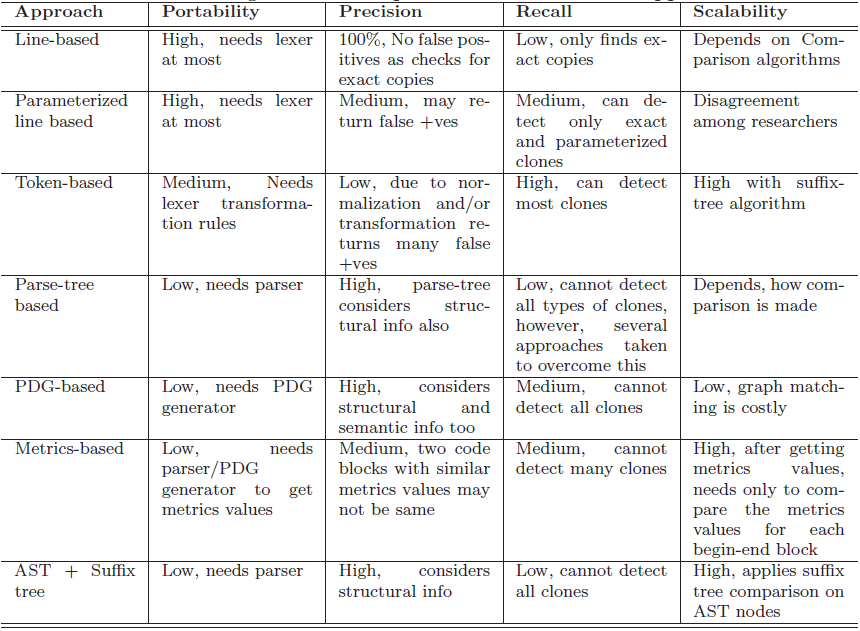
\includegraphics[width=.9\textwidth]{cmp.png}
\end{center}
\end{frame}

\part{Researches about Code Clones}
\frame{\partpage}

\section{Removal, Avoidance and Management of Code Clones}
\begin{frame}
\frametitle{\secname}
\begin{block}{}
\begin{enumerate}
  \item Removal of Code Clones
  \begin{itemize}
    \item remove clones through ${(automatic)\ refactoring}$
  \end{itemize}
  \item Avoidance of Code Clones
  \begin{itemize}
    \item use a clone detection tool in normal development process
    \item $preventive\ control$ ensures every added function is not a clone
    \item $problem\ mining$ ensures modification to a function propagated
    to all of its similar functions
  \end{itemize}
  \item Management of Code Clones
  \begin{itemize}
    \item \structure{track} existing clones either
    in $individual\ version$ or $evolving\ versions$
  \end{itemize}
  \end{enumerate}
\end{block}
\end{frame}

\section{Evolution Analysis of Clones}
\begin{frame}
\frametitle{\secname}
\begin{block}{}
There are several studies that look at how clones \structure{evolve} in
different versions of a software system.
\end{block}
\begin{itemize}
  \item Evaluating \structure{whether a clone detection tool helps} when
  integrated with the development process.
  \item \structure{Monitoring \& predicting} the evolution of clones
  \item Analysis \structure{clone genealogies}, the evolution of clone groups over
  different versions of a software system.
\end{itemize}
\end{frame}

\section{Quality Analysis Based on Code Clones}
\begin{frame}
\frametitle{\secname}
\begin{block}{}
While it is frequently stated that clones negatively affect
software maintenance, there is \structure{not much} proof that they
really do.
\end{block}
\pause
\begin{block}{One study by Monden et al.}
\begin{itemize}
  \item Conducted for evaluating relation between clones \& software
  quality attributes(reliability \& maintainability)
  \pause
  \item \alert{Modules\slash files with code clones are on average 1.7 times more
  reliable than those without!}
  \item Files/modules with code clones are less maintainable
than those without.
\end{itemize}
\end{block}
\end{frame}

\section{Open Problems for Future Research}
\begin{frame}
\frametitle{\secname}
\begin{itemize}
  \item Types and Taxonomies of Clones(Formal definition,Clone length,Relevance
  ranking\ldots)
  \item Evaluation of Clone Detection Techniques
  \alert{\item Better Clone Detection Techniques
  \begin{itemize}
    \item less false positive/negative
    \item Especial treatment for detecting $Type\
    \uppercase\expandafter{\romannumeral3} ,Type\
    \uppercase\expandafter{\romannumeral4}$ clones
    \item Semantic clone detection tool
  \end{itemize}}
  \item Empirical Studies in Clone Detection Research
\end{itemize}
\end{frame}

\part{What I Want to Research into \& What I'm Confused}
\frame{\partpage}
\section{Some facts}

\begin{frame}
\frametitle{Is code clone a common practice in C,Java and Python?}
\begin{block}{An Answer from stackoverflow}
\begin{itemize}
  \item Code cloning is \structure{extremely common} no matter what programming
  language is used, yes, even in C, Python and Java.
  \item I \alert{don't} think clones are bad, because of the code reuse effect.
  I think what is bad is not \structure{managing} them.
  \item In any software system of $100K\ SLOC$ or more, at least $10\%$ of the code is
  cloned.It tends to be \structure{worse} in older conventional applications.
\end{itemize}
\rightline{---Ira Baxter}
\end{block}
\end{frame}

\begin{frame}
\frametitle{A Result about Frequency and Risks of Changes to Clones}
\begin{itemize}
  \item For $87.8\%$ of the clones that \structure{never changed} or
  \structure{changed once}, removal would not have been beneficial
  \item $14.8\%$ of all changes were unintentionally inconsistent
  \item Regarding severity
  \begin{enumerate}
    \item $11.8\%$ of the unwanted inconsistencies had
    only low severity whereas
    \item only $3.0\%$ of all changes were found to have high
    severity.
  \end{enumerate}
\end{itemize}
\end{frame}

\section{My thoughts}
\begin{frame}
\frametitle{\secname}
\begin{block}{Motivation}
\begin{itemize}
  \item Code clones are omnipresent in \structure{original development process}
  \item There are excellent code fragments for programmers' reuse
  \item Clones may introduce new bugs
  \begin{itemize}
    \item shadowed variables
    \item variable reassignment
    \item \ldots
  \end{itemize}
  \item Testing all clone fragments is costly
\end{itemize}
\end{block}
\pause
\vskip11pt
\centerline{\alert{Test one clone, generate less test cases for others}}
\end{frame}

\begin{frame}
\frametitle{Mind Map}
\begin{center}
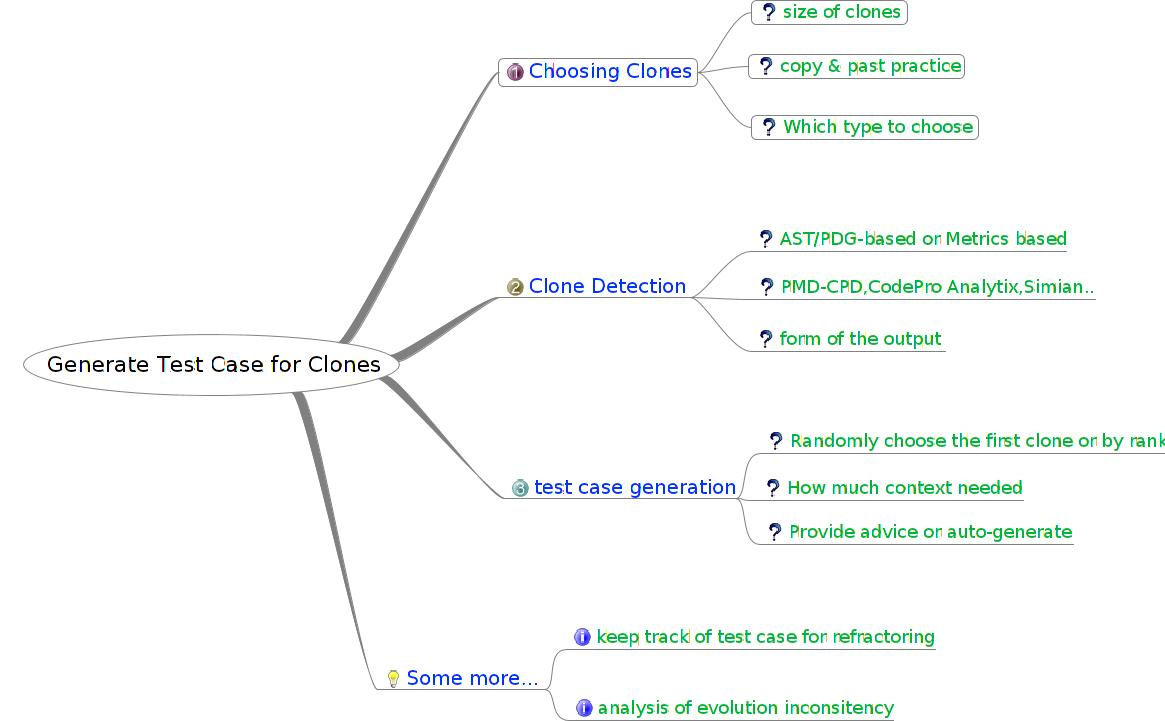
\includegraphics[width=.9\textwidth]{Generate_Test_Case_for_Clones.jpeg}
\end{center}
\end{frame}

\begin{frame}
\frametitle{Current Plan}
\begin{columns}
\column{.35\textwidth}
\begin{enumerate}
  \item Select one kind of clone detection tool such as PMD:CPD
  \vskip11pt
  \item Find some bug patterns introduced by code clones manually 
    \vskip11pt
  \item Hack the source code of the detection tool to make the output
  suitable for test generation
\end{enumerate}
\column{.65\textwidth}
\footnotesize
{
\begin{block}{PMD analyzer}
\begin{itemize}
  \item Uses JavaCC parser generator in conjunction with an EBNF grammar and JJTree
  to parse Java source code into an AST
  \item CPD is included to detect duplicate code
\end{itemize}
\end{block}
\begin{block}{CPD detector}
\begin{itemize}
  \item 2 kind of parsers availables
  \begin{itemize}
    \item One basic parser, easily tuneable to any language
    \item One based on (Java) AST but far more accurate
    \end{itemize}
  \item Detect clones with a minimal tile size in a project
  \item Output:possible duplicate code
\end{itemize}
\end{block}
}
\end{columns}
\end{frame}

\begin{frame}
\frametitle{Other Possible Difficulties}
\begin{columns}
\column{.45\textwidth}
\begin{itemize}[<+->]
  \item How to use the result of detection for test case generation?
  \item What if the cost is higher when compared to general testing?
  \item What about the precision and soundness?
  \item What's the practical use?
\end{itemize}
\column{.5\textwidth}
\begin{center}

\includegraphics[width=\textwidth]{help.png}
\end{center}
\end{columns}
\end{frame}

\end{document}
